\documentclass[english,notitlepage]{revtex4-1}
\usepackage{physics,amssymb}
\include{amsmath}
\usepackage{graphicx} % Required for inserting images
\usepackage{float}
\usepackage{parskip}

\begin{document}

\title{Project 2 - Computational Physics FYS3150/FYS4150 } 
\author{Émilie Valle, Josef Ayman}          
\date{\today}                             
\noaffiliation          % ignore this, but keep it.

\maketitle

\textit{GitHub repo: \href{https://github.uio.no/josefam/FYS3150}{github.uio.no/josefam/FYS3150}}

\section{Problem 1}
We have to show that eq(1) can be written as eq(2).

\begin{equation}
    \gamma\frac{d^2u(x)}{dx^2}=-Fu(x)
\end{equation}
\begin{equation}
    \frac{d^2u(\hat{x})}{d\hat{x}^2}=-\lambda u(\hat{x})
\end{equation}
with $\hat{x}=\frac{x}{L}$ and $\lambda=\frac{FL^2}{\gamma}$\\

We can begin from the end to back up in the beginning.
\begin{equation}
    \frac{d^2u(\hat{x})}{d\hat{x}^2}=-\lambda u(\hat{x})
\end{equation}
\begin{equation}
    \frac{d^2u(\frac{x}{L})}{d(\frac{x}{L})^2}=-\frac{FL^2}{\gamma}u(\frac{x}{L})
\end{equation}
\begin{equation}
    \gamma\frac{d^2u(x)}{dx^2}\frac{L^2}{L}=-F\frac{L^2}{L}u(x)
\end{equation}
\begin{equation}
    \gamma\frac{d^2u(x)}{dx^2}=-Fu(x)
\end{equation}

\bigbreak
\section{Problem 2}
As asked, we have set up the tridiagonal 6x6 matrix and solves $A\overrightarrow{v}=\lambda\overrightarrow{v}$ using Armadillo. Then, we have checked that the eigenvalues and eigenvectors agrees with the analytical result for $N=6$. The thing with scaling of vectors has been done with the normalization as discussed in the introduction of the project.

And then, we have found that the checking is good and all the values are quite the same.

\bigbreak
\section{Problem 3}
a) The function coded here has permitted to find the largest off-diagonal element and to give its absolute value using Armadillo.

b) With the following matrix :

\begin{gather}
\begin{bmatrix}
    1 & 0 & 0 & 0.5\\
    0 & 1 & -0.7 & 0\\
    0 & -0.7 & 1 & 0\\
    0.5 & 0 & 0 & 1\\
\end{bmatrix}
\end{gather}\\
we can see that, the function has found $-0.7$ as largest off-diagonal element and $0.7$ as its absolute value, which is the right answer.

\bigbreak
\section{Problem 4}
a) The function coded here, using the code snippets can solve the following equation with Jacobi's rotation algorithm. Note that, the suggested code structure has been used but not the helper functions.
\begin{equation}
    A\overrightarrow{v}=\lambda\overrightarrow{v}
\end{equation}

b) With this code, we have check if the eigenvalues and eigenvectors agree with the analytical results for $N=6$.

We can see in both case that, the difference between the analytical and the Jacobi's method is very small. For the eigenvectors, we have a difference like $1\times10^{-12}$ and for the eigenvalues, $1\times10^{-14}$.

\bigbreak
\section{Problem5}
a) With the Jacobi's method, we can run our program with different choices of N and see the number of required transformation we need to solve eq(8).

Here the table of results : (with i as iterations)\\
$\left\{
    \begin{array}{ll}
        N = 10, i = 137\\
        N = 20, i = 655\\
        N = 40, i = 2762\\
        N = 80, i = 11214\\
        N = 160, i = 45319\\
        N = 320, i = 182906\\
    \end{array}
\right.$

We can then, do the plot with a linear scale and with a log scale.
\begin{figure} [H]
    \centering
    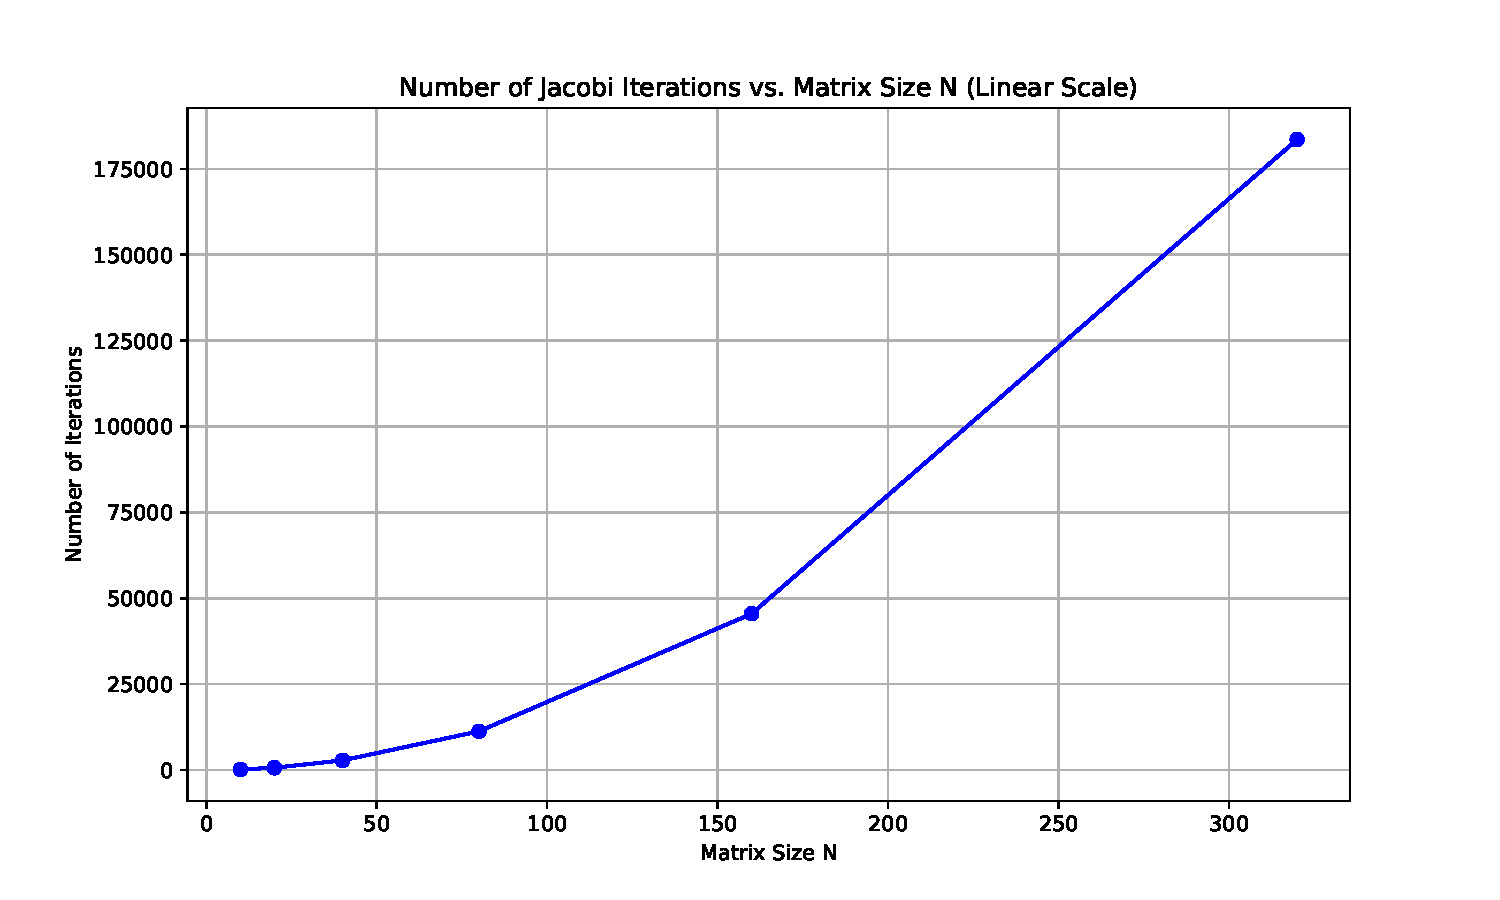
\includegraphics[width=0.75\linewidth]{problem5/jacobi_iterations_linear.pdf}
    \caption{Plot of Jacobi's iterations in linear scale}
    \label{fig:enter-label}
\end{figure}

\begin{figure} [H]
    \centering
    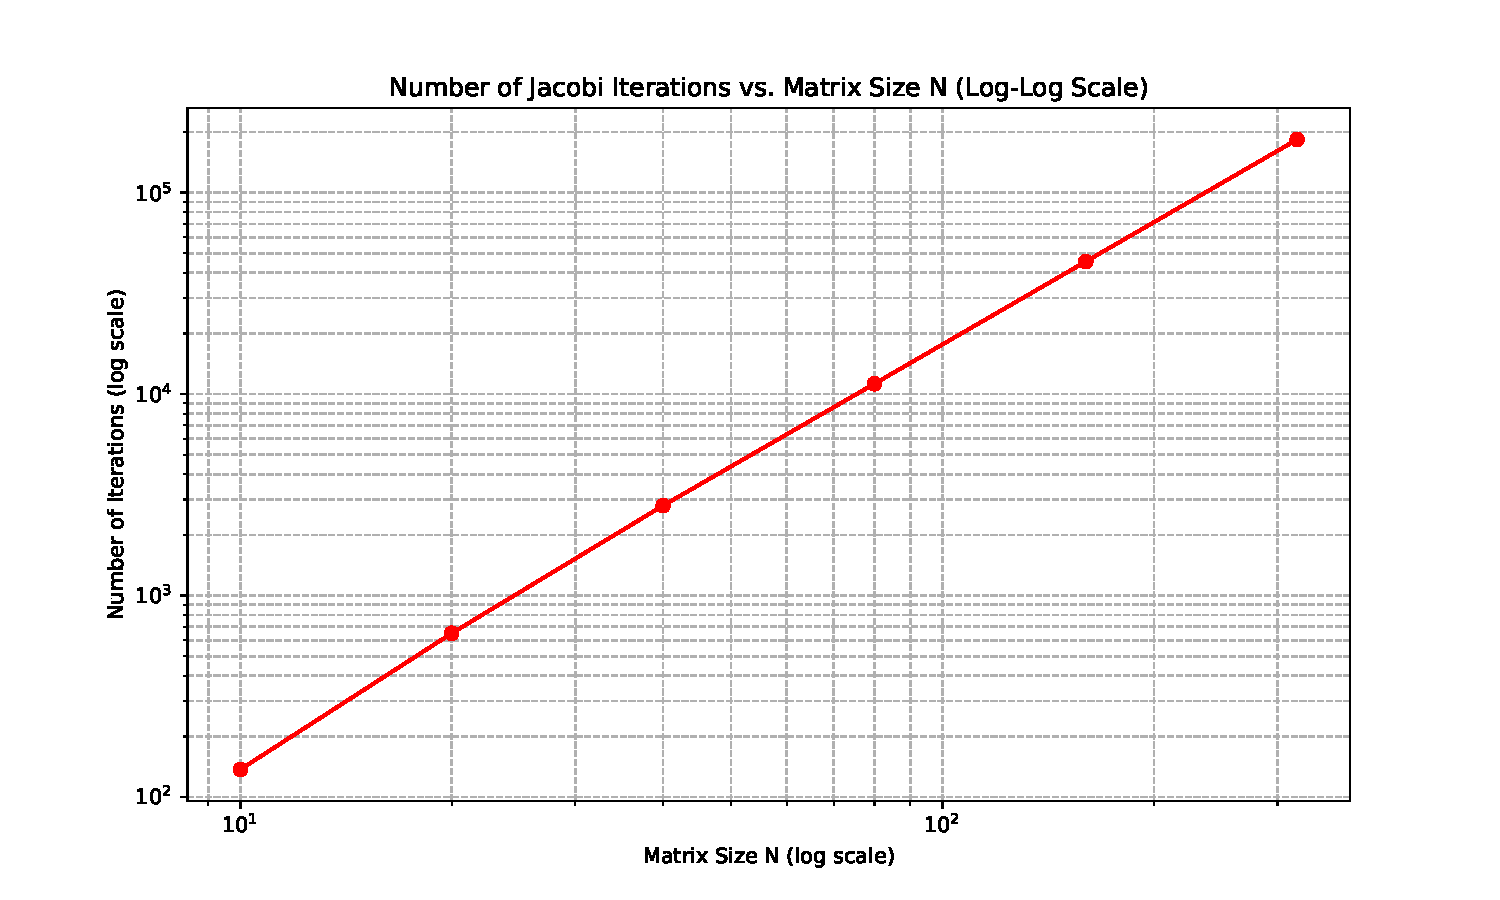
\includegraphics[width=0.75\linewidth]{problem5/jacobi_iterations_loglog.pdf}
    \caption{Plot of Jacobi's iterations in log scale}
    \label{fig:enter-label}
\end{figure}

And then, try to find a function to fit with the plot. With this, we have the scale of the number of required transformations with the matrix N size when we use our code to solve eq(8).
\begin{figure} [H]
    \centering
    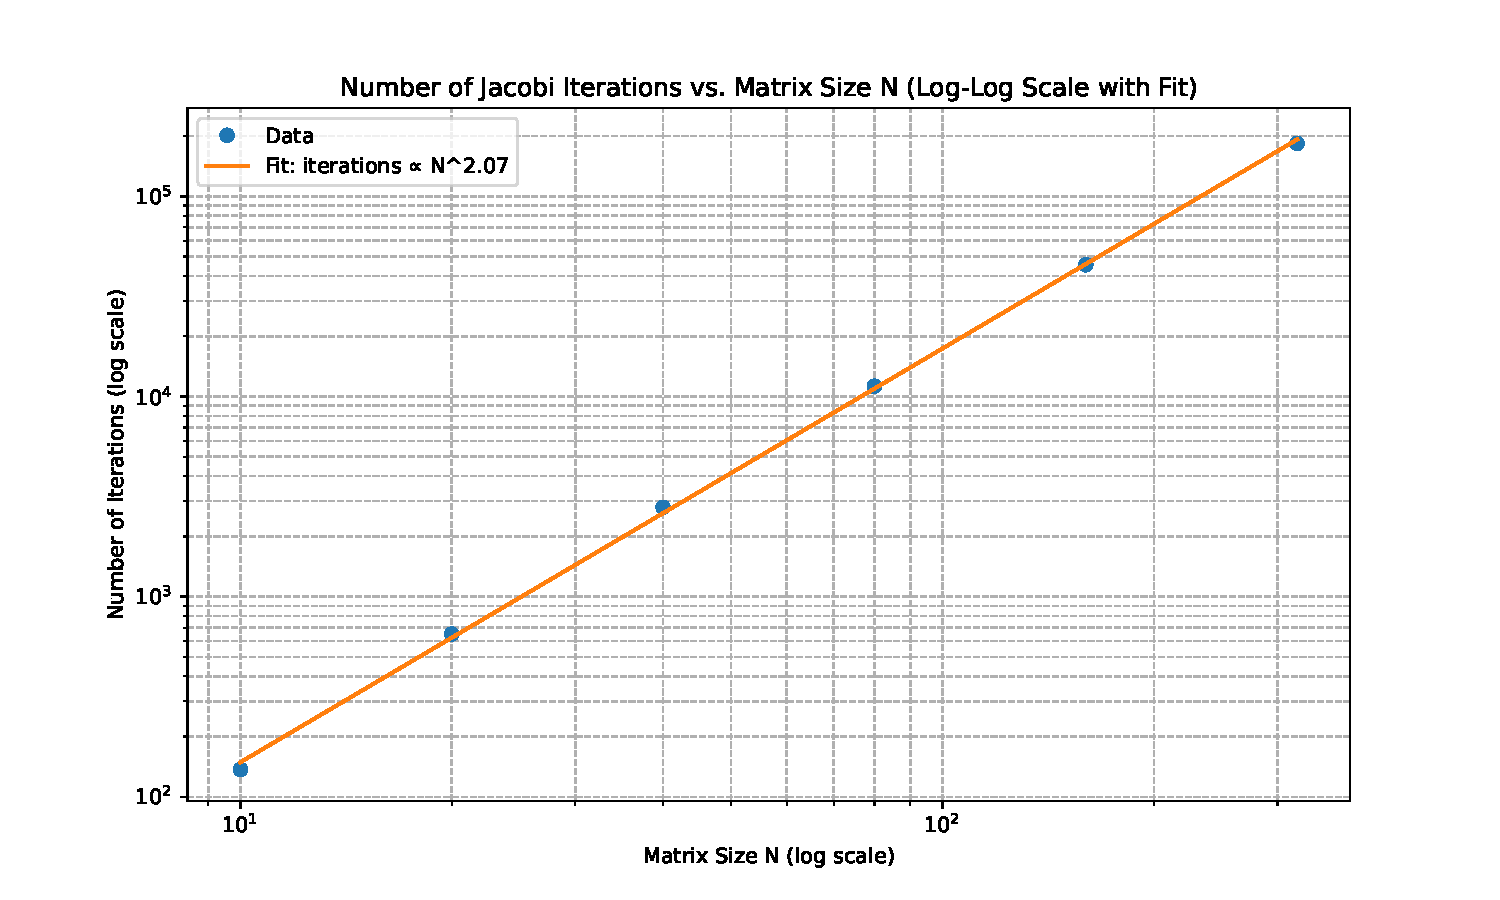
\includegraphics[width=0.75\linewidth]{problem5/jacobi_iterations_loglog_fit.pdf}
    \caption{Fit function with log scale}
    \label{fig:enter-label}
\end{figure}
So, the scale is $N*2.07$ in log scale.
\subsection*{}
b) 
% Josef's Notes:
For a dense symmetric matrix, we would expect the scaling behavior to be similar or even worse than \(O(N^2)\), due to the larger number of off-diagonal elements that need to be eliminated.

% \textbf{Explanation:}
\begin{itemize}
    \item The Jacobi algorithm does not take advantage of the sparsity of the initial matrix.
    \item Even starting with a sparse matrix, the rotations introduce non-zero elements (fill-in effect), effectively making the matrix dense as the algorithm progresses.
    \item Therefore, the scaling behavior for a dense matrix would also be quadratic or worse.
\end{itemize}

\textbf{Scaling behavior:}
% -What scaling behavior would you expect to see if \( \mathbf{A} \) was a dense matrix?

\begin{itemize}
    \item In a dense matrix, the number of off-diagonal elements is \( N(N - 1)/2 \), which scales as \( O(N^2) \).
    \item Each Jacobi rotation zeroes out one off-diagonal element.
    \item In the worst case, we may need to apply a number of rotations proportional to the number of off-diagonal elements.
    \item Each rotation involves updating \( O(N) \) elements in the matrix and the eigenvector matrix.
    \item The total cost is roughly \( O(N^3) \) for dense matrices.
\end{itemize}

\section{Problem 6}
\subsection*{}
a) With our Jacobi code, we have made a plot of the three eigenvectors corresponding to the three lowest eigenvalues comparing with the analytical answers.
\begin{figure} [H]
    \centering
    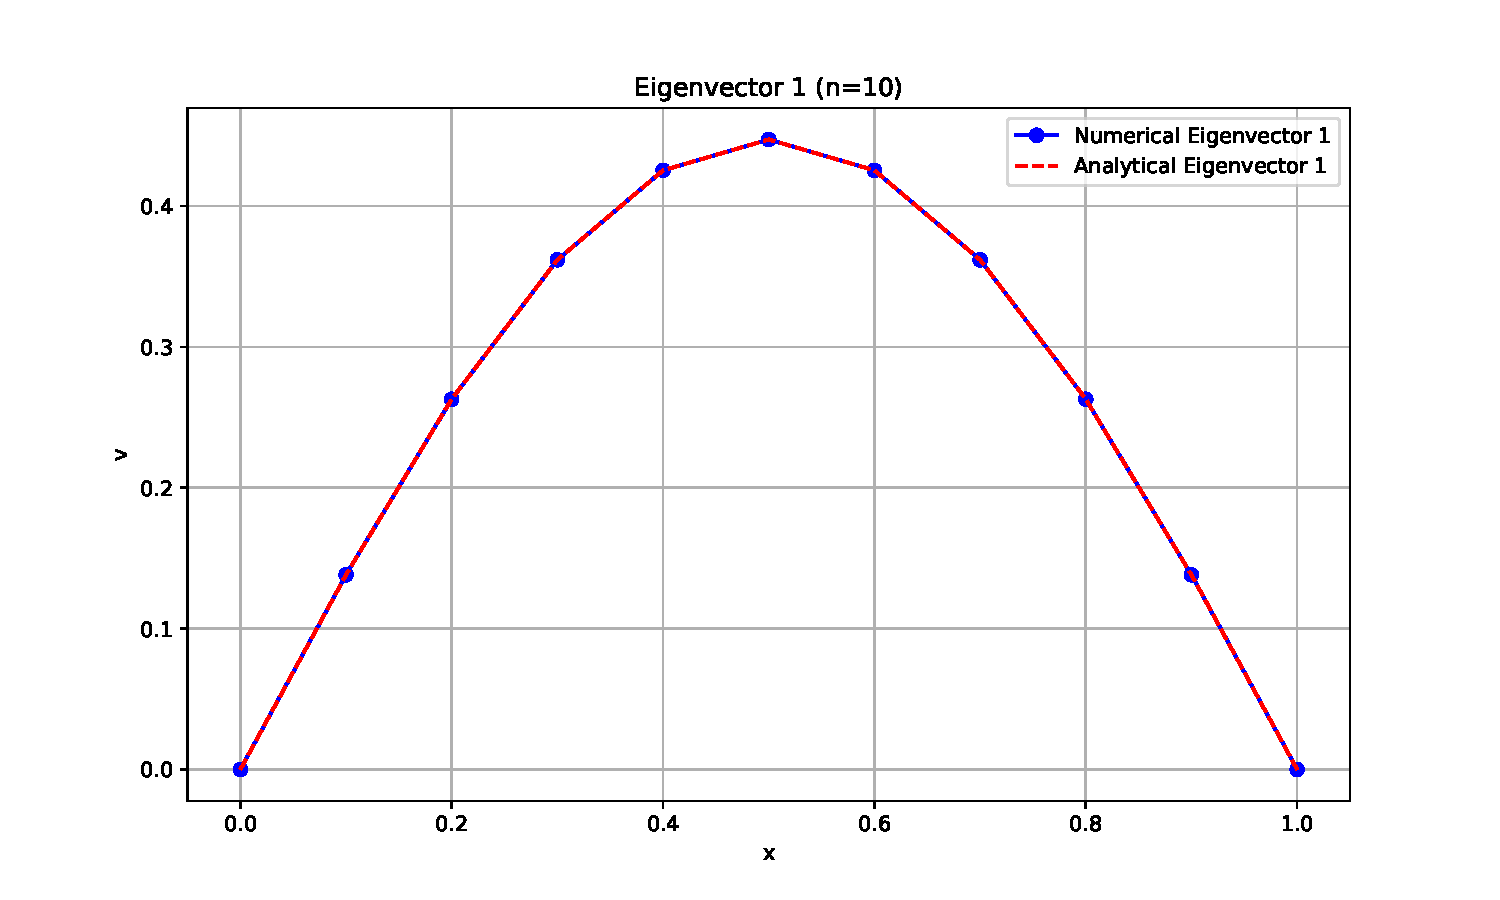
\includegraphics[width=0.75\linewidth]{problem6/eigenvector1_n10.pdf}
    \label{fig:enter-label}
\end{figure}
\begin{figure} [H]
    \centering
    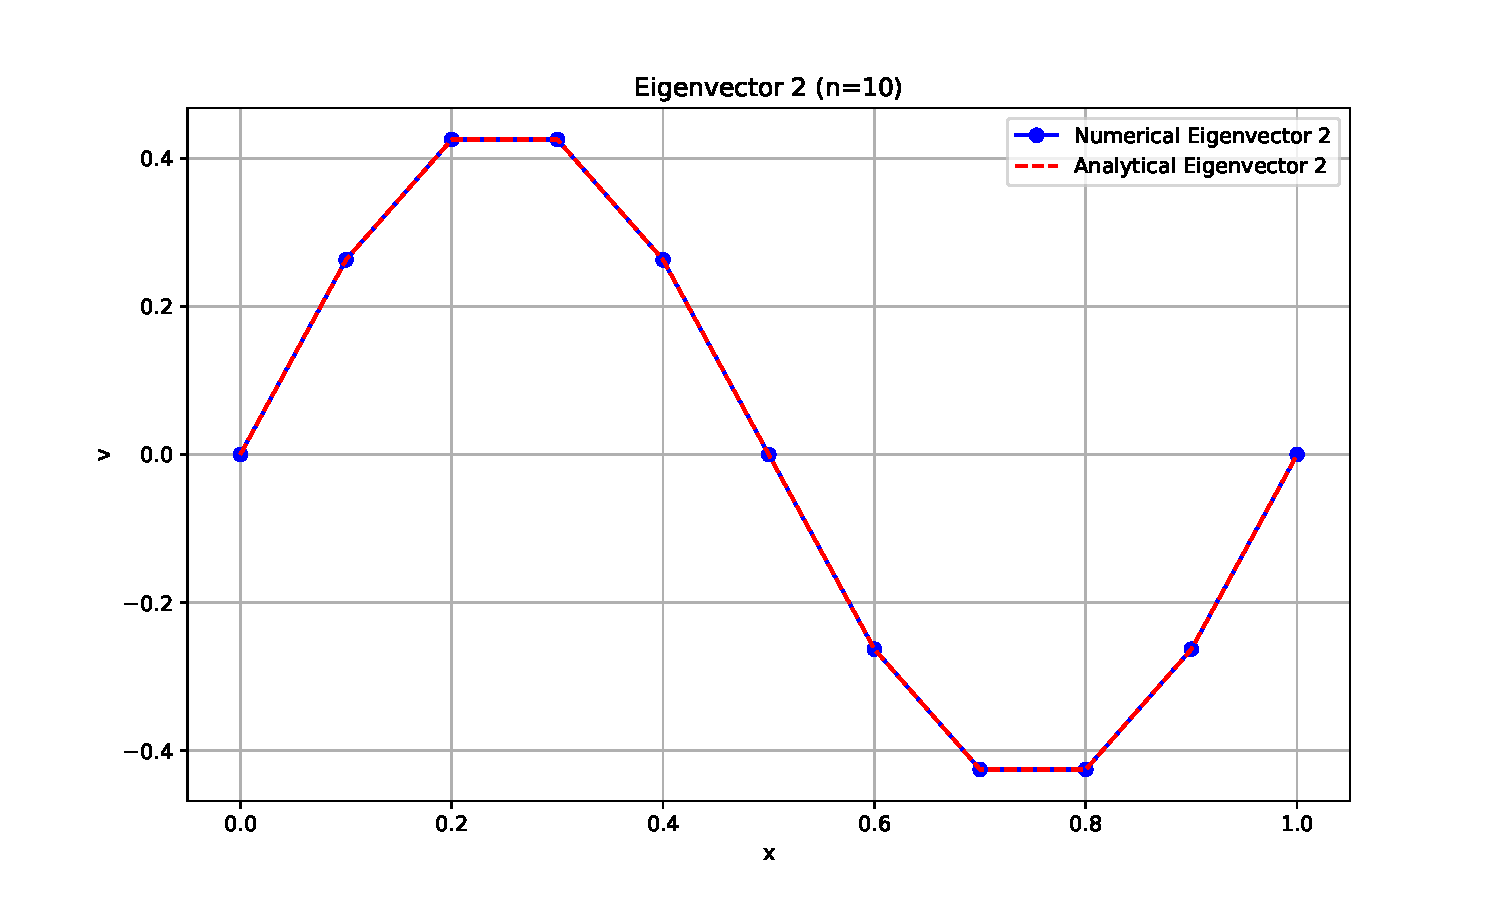
\includegraphics[width=0.75\linewidth]{problem6/eigenvector2_n10.pdf}
    \caption{Second eigenvector with n = 10}
    \label{fig:enter-label}
\end{figure}
\begin{figure} [H]
    \centering
    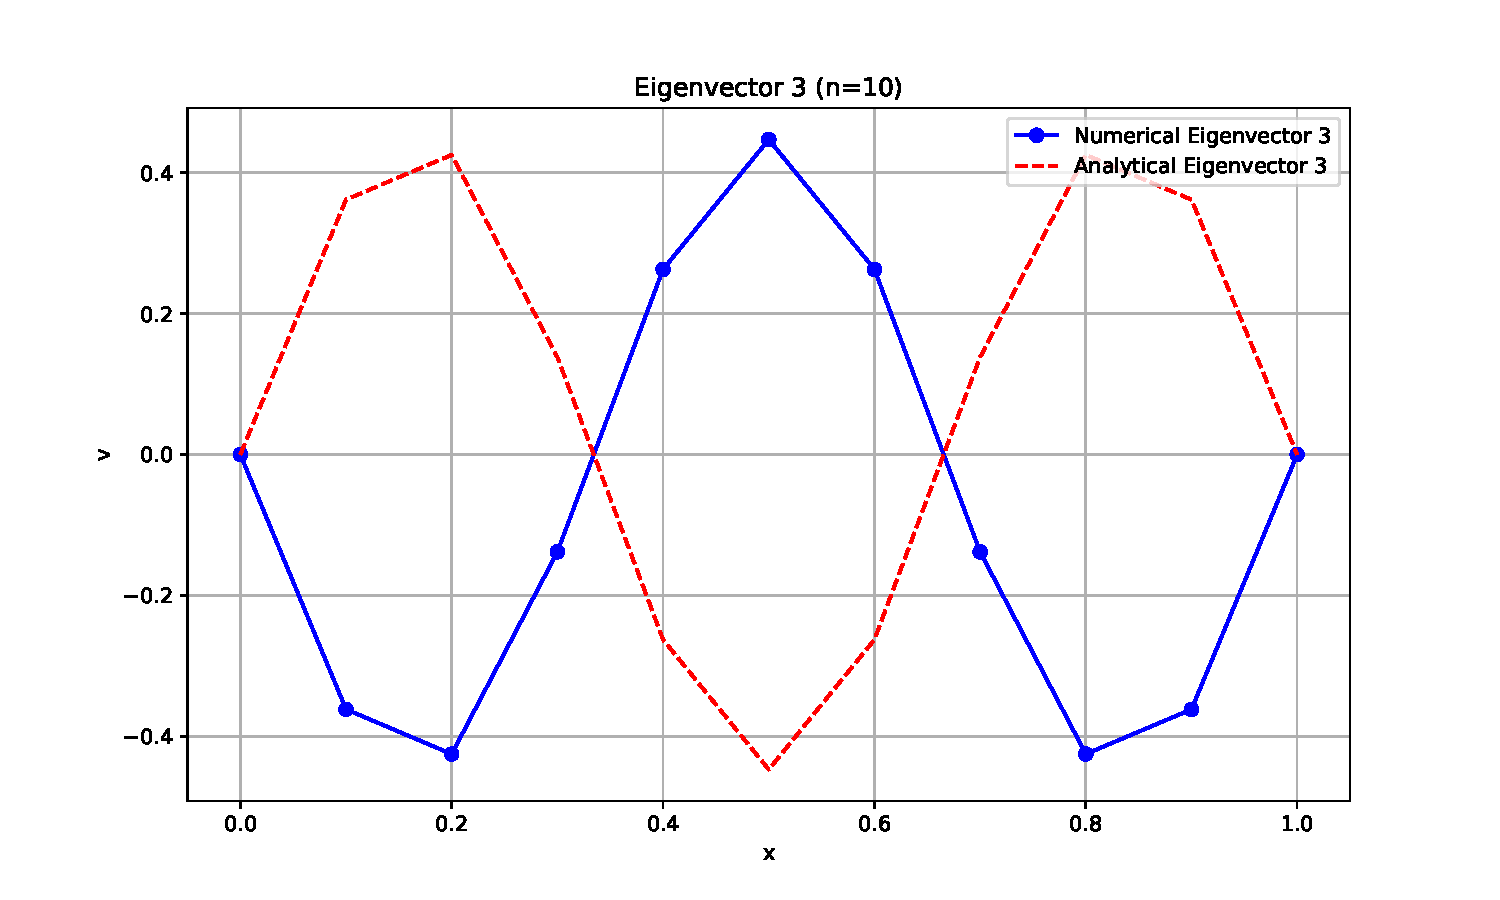
\includegraphics[width=0.75\linewidth]{problem6/eigenvector3_n10.pdf}
    \caption{Third eigenvector with n = 10}
    \label{fig:enter-label}
\end{figure}

\subsection*{}
b) For the $n = 100$, here the plots.

\begin{figure} [H]
    \centering
    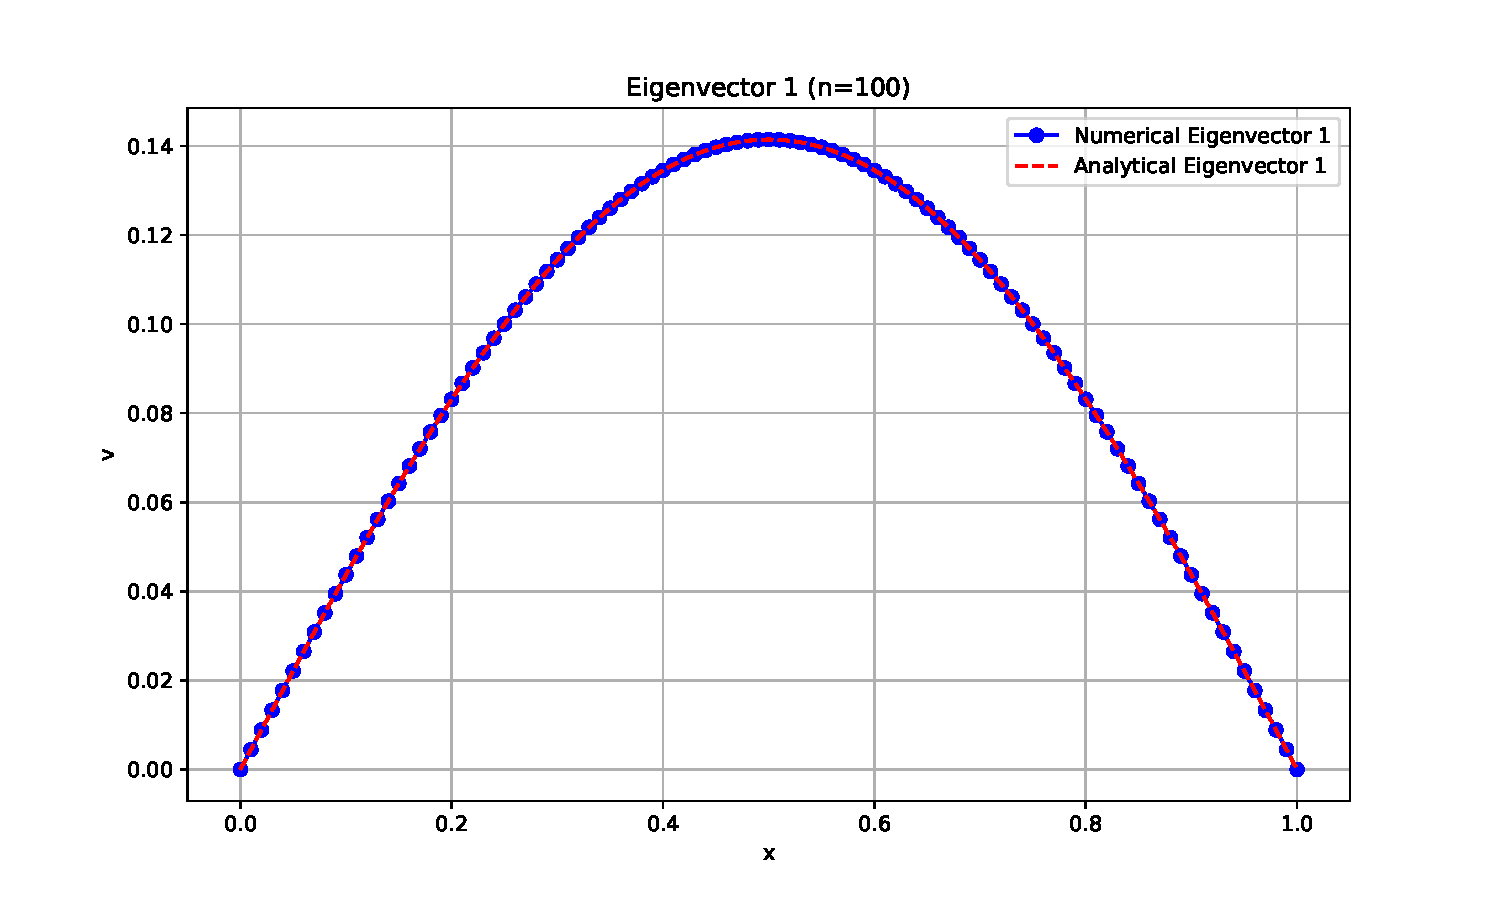
\includegraphics[width=0.75\linewidth]{problem6/eigenvector1_n100.pdf}
    \caption{First eigenvector with n = 100}
    \label{fig:enter-label}
\end{figure}
\begin{figure} [H]
    \centering
    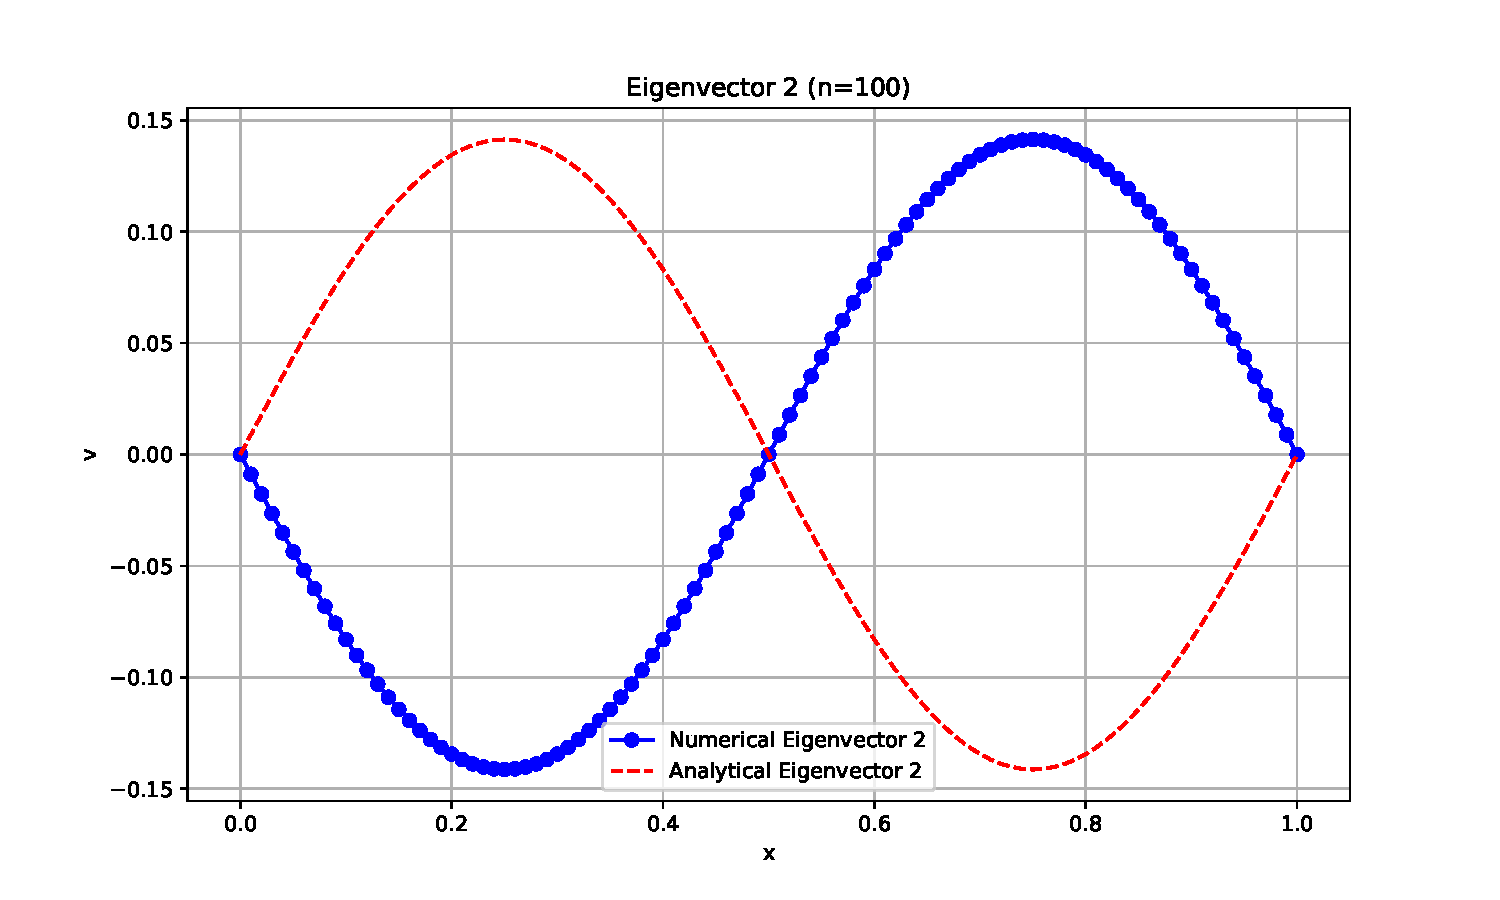
\includegraphics[width=0.75\linewidth]{problem6/eigenvector2_n100.pdf}
    \caption{Second eigenvector with n = 100}
    \label{fig:enter-label}
\end{figure}
\begin{figure}
    \centering
    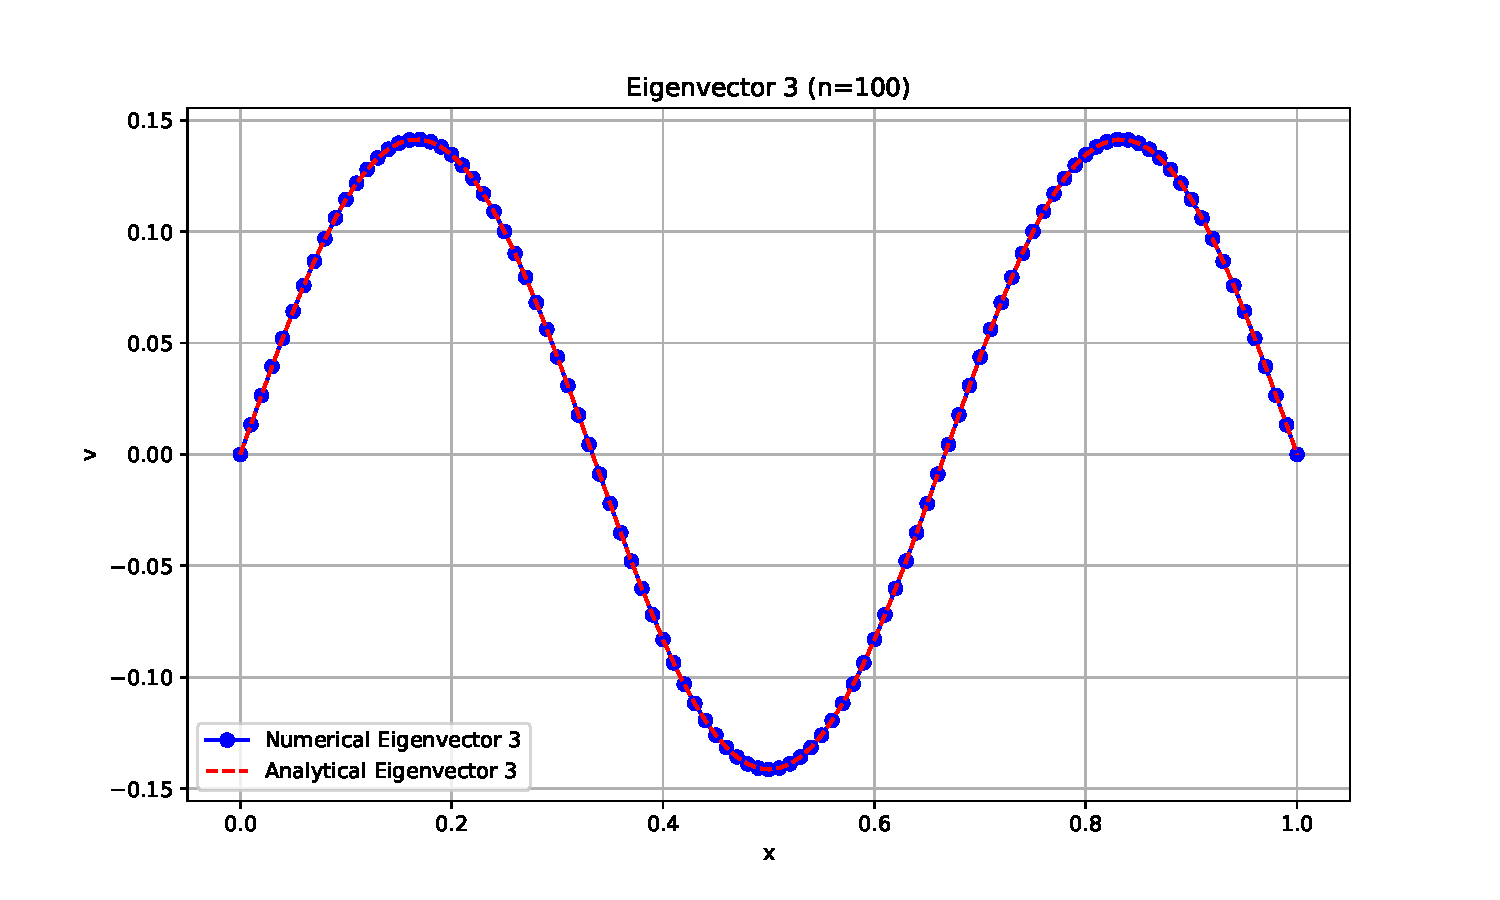
\includegraphics[width=0.75\linewidth]{problem6/eigenvector3_n100.pdf}
    \caption{Third eigenvector with n = 100}
    \label{fig:enter-label}
\end{figure}

\end{document}
